%Part of/Parte di https://github.com/f-dinucci/appuntiMeccanicaFluidi/
%License/Licenza Creative Commons Attribution-ShareAlike 4.0 International (CC BY-SA 4.0) - attribution/attribuzione Francesco Di Nucci
%See also/Vedere anche https://creativecommons.org/licenses/by-sa/4.0/ and/e https://creativecommons.org/licenses/by-sa/4.0/legalcode
%
\section{Correnti a basso numero di Reynolds}
\subsection{Approssimazioni per Reynolds piccolo}
Nel caso in cui invece le dimensioni siano dello stesso ordine di grandezza ma il numero di Reynolds sia piccolo si hanno delle semplificazioni differenti.
Si parte dalle equazioni di Stokes:
%
	\begin{equation*}
		\left\{
			\begin{gathered}
				u_x + u_y = 0\\
				u_t + p_x = u_{xx} + u_{yy}\\
				v_t + p_y = v_{xx} + v_{yy}
			\end{gathered}
		\right.
	\end{equation*}
%
Si richiama poi la funzione di corrente:
%
	\begin{equation*}
		\left\{
			\begin{gathered}
				\psi_y = u\\
				\psi_x = -v
			\end{gathered}
		\right.
	\end{equation*}
%
Con la funzione di corrente si può arrivare a due equazioni (quella di continuità è automaticamente risolta):
%
	\begin{equation*}
		\left\{
			\begin{gathered}
				\psi_{yt} + p_x = \psi_{xxy} + \psi_{yyy}\\
				- \psi_{xt} + p_y = - \psi_{xxx} - \psi_{xyy}
			\end{gathered}
		\right.
	\end{equation*}
%
Si può poi derivare la prima equazione rispetto a y e la seconda rispetto ad x, per avere lo stesso termine riguardante la pressione:
%
	\begin{equation*}
		\left\{
			\begin{gathered}
				\psi_{yyt} + p_{xy} = \psi_{xxyy} + \psi_{yyyy}\\
				- \psi_{xxt} + p_{xy} = - \psi_{xxxx} - \psi_{xxyy}
			\end{gathered}
		\right.
	\end{equation*}
%
Sottraendo una dall'altra:
	\begin{equation*}
		{\left( \psi_{xx} + \psi_{yy} \right)}_t  = \psi_{xxxx} + 2 \psi_{xxyy} + \psi_{yyyy}\\
	\end{equation*}
%
Richiamando l'operatore laplaciano:
%
	\begin{equation*}
		\laplacian = \pdv[2]{x} + \pdv[2]{y}
	\end{equation*}
%
Si arriva quindi ad una equazione in una incognita:
%
	\begin{equation*}
		{\left( \laplacian{\psi} \right)}_t = \laplacian{ \laplacian{ \psi } }
	\end{equation*}
%
Volendo è possibile introdurre la vorticità, non conviene perché aumentano le incognite, ma è un collegamento interessante:
%
	\begin{equation*}
		\begin{gathered}
			\laplacian{\psi} = u_y - v_x = - \omega\\
			\omega_t = \laplacian{ \omega }
		\end{gathered}
	\end{equation*}
%

\subsection{Cilindro in fluido}
Una delle applicazioni d'interesse è quella di un cilindro immerso in un fluido, per calcolare ad esempio la resistenza offerta.
Si suppone di essere in un caso stazionario e si usa un sistema di coordinate cilindriche.
Il raggio del cilindro viene visto come unitario (in altre parole lo si prende come grandezza di riferimento).
 %
	\begin{figure}[ht]
		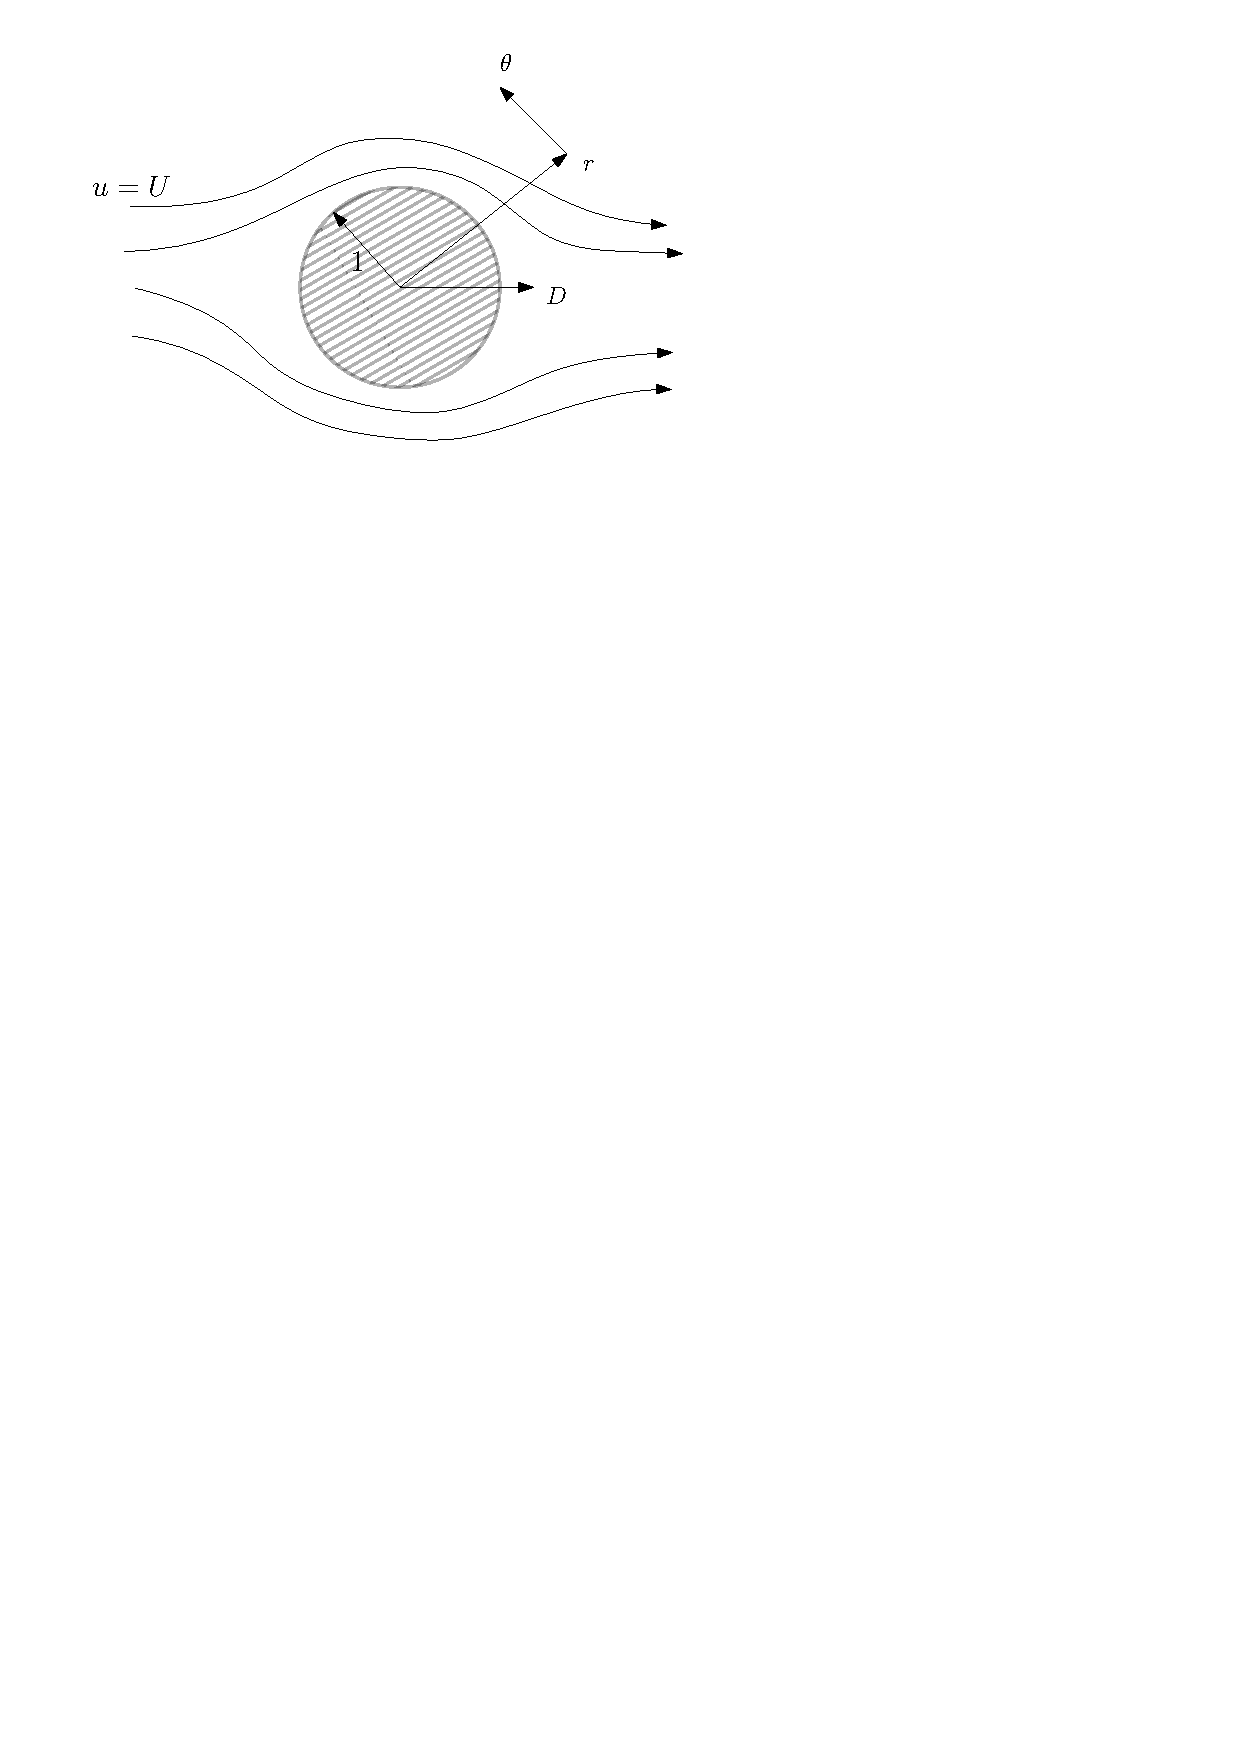
\includegraphics[scale=0.7]{./6.4 Correnti a basso numero di Reynolds/6.4-1}
		\centering
		\caption{Cilindro in fluido}
	\end{figure}
%
Si prende la condizione sulla velocità ad infinito in coordinate cilindriche:
%
	\begin{equation*}
		\begin{gathered}
			u = U\\
			\psi = u_y = U r \sin{\theta}
		\end{gathered}
	\end{equation*}
%
Per un'equazione alle derivate parziali non ci sono metodi di risoluzione fissi, in questo caso si suppone che la soluzione sia funzione di $r$ e $\theta$:
%
	\begin{equation*}
		\psi = F(r) \sin{\theta}
	\end{equation*}
%
Da cui si trovano le condizioni al contorno:
%
	\begin{equation*}
		\begin{gathered}
			r \rightarrow \infty \quad F = U r\\
			r \rightarrow 1 \quad F = 0 \quad F' = 0
			\end{gathered}
\end{equation*}
%
Si verifica poi se l'equazione ammetta una soluzione come quella ipotizzata:
%
	\begin{equation*}
		\begin{gathered}
			\laplacian{\psi} = \frac{1}{r} \pdv{\left( r \psi_r \right)}{r}  + \frac{1}{r^2} \psi_{\theta \theta} =\\
			= \frac{1}{r} (r F')' \sin{\theta} - \frac{F}{r^2} \sin{\theta} = \left[ \frac{1}{r} (r F')' - \frac{F}{r^2} \right] \sin{\theta}
		\end{gathered}
	\end{equation*}
%
È veramente il prodotto di due funzioni, calcolandone il laplaciano risulta:
%
	\begin{equation*}
			\laplacian{\laplacian{\psi}} = \left[ \frac{1}{r} \pdv{r} (r \pdv{r})  - \frac{1}{r^2} \right] \left[ \frac{1}{r} (r F')' - \frac{F}{r^2} \right] \sin{\theta} = 0
	\end{equation*}
%
È un'equazione omogenea, ha soluzioni in casi particolari, in questo caso ha soluzioni del tipo $F = r^a$:
%
	\begin{equation*}
			\left[ \frac{1}{r}  \pdv{r} (r \pdv{r}) - \frac{1}{r^2} \right] \left[ a^2 r^{a-2} - r^{a - 2} \right] = (a^2 - 1) [{(a -2)}^2 - 1] r^{a-4} = 0
	\end{equation*}		
%	
Le soluzioni sono:
%
	\begin{equation*}	
		\begin{gathered}
			a = \left\{
				\begin{aligned}
					-1\\
					+1\\
					+1\\
					+3
				\end{aligned}
				\right.
		\end{gathered}
	\end{equation*}
%
Da cui, considerata la presenza di una radice doppia, le soluzioni sono:
%
	\begin{equation*}
		\left\{
			\begin{aligned}
				r^{-1}\\
				r\\
				r \log{r}\\
				r^3
			\end{aligned}
		\right.
	\end{equation*}
%
Quindi:
%
	\begin{equation*}
		\psi = \left( A r^{-1} + B r + C r \log{r} + D r^3 \right) \sin{\theta}	
	\end{equation*}
%
È ora possibile imporre le condizioni al contorno:
%
	\begin{equation*}
		\begin{gathered}
			F(1) = 0\\
			\quad F'(1) = 0\\
			F(r \rightarrow \infty) \rightarrow U r
		\end{gathered}
	\end{equation*}
%
Dato che ad infinito la velocità deve tendere ad $U r$, le potenze più grandi devono essere nulle, altrimenti la velocità ``esploderebbe'', quindi $C = D = 0$.
Per rispettare la condizione sulla velocità poi $B = U$.
Questo lascia una sola costante ancora da determinare, $A$, con due condizioni al contorno.
Quindi non è possibile trovare una soluzione, il problema presenta un paradosso e non è risolvibile.

Questo vuol dire che non esiste un flusso \textit{di Stokes} attorno ad un cilindro, non che non esiste un flusso \textit{in generale}.
Ci si rende conto che non è possibile trascurare del tutto il numero di Reynolds, questo si risolve con una approssimazione.
Si può dimostrare che:
%
	\begin{equation*}
		u \sim U + o\left( \frac{1}{r} \right)
	\end{equation*}
%
 %
	\begin{figure}[ht]
		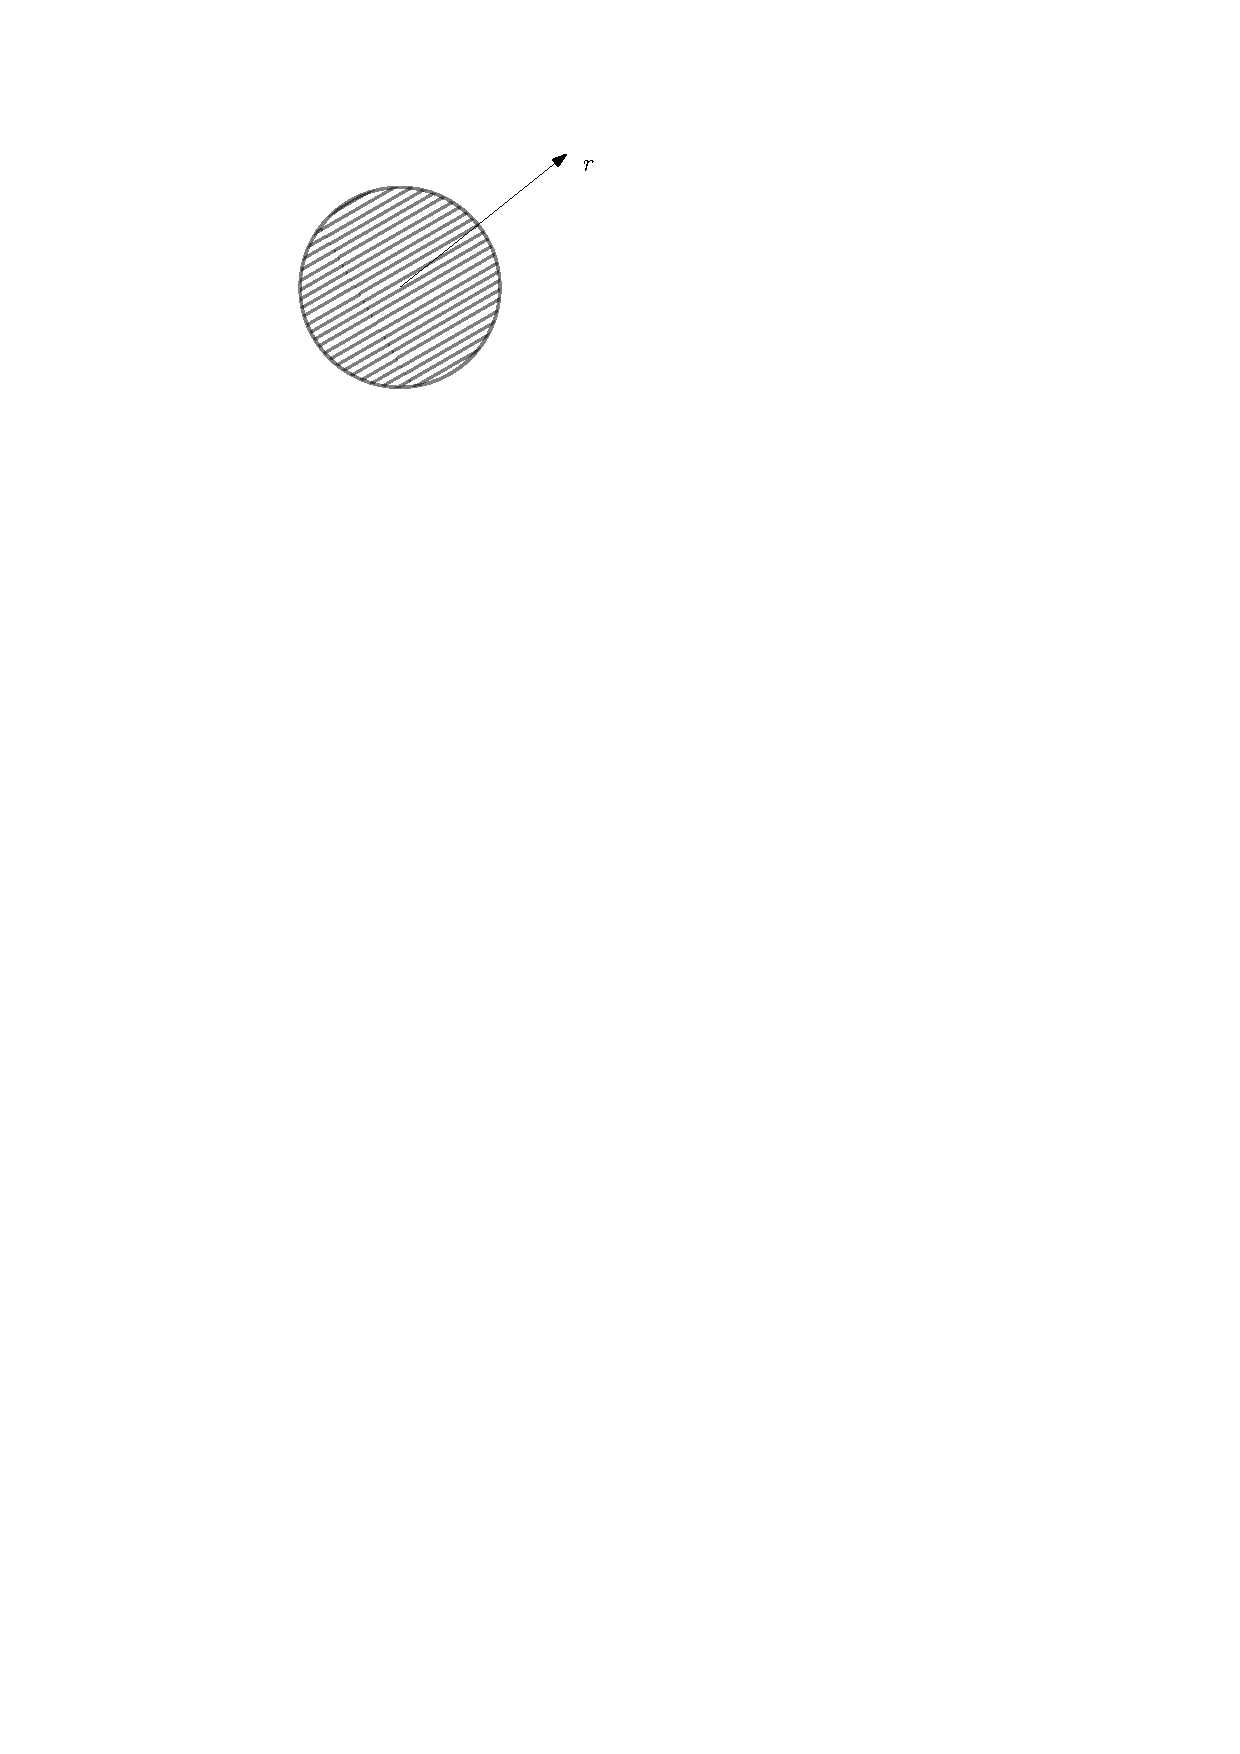
\includegraphics[scale=0.7]{./6.4 Correnti a basso numero di Reynolds/6.4-2}
		\centering
		\caption{Ci si pone ad una certa distanza dal cilindro}
	\end{figure}
%
Nei pressi del corpo si fa un'approssimazione detta approssimazione di Oseen:
%
	\begin{equation*}
		u u_x \rightarrow U u_x
	\end{equation*}
%
Per cui:
%
	\begin{equation*}
		U u_x + p_x = \frac{1}{R_e} (u_{xx} + u_{yy})
	\end{equation*}
%
Si può poi trovare che la resistenza come ordine di grandezza è:
%
	\begin{equation*}
		D \sim \frac{1}{\log{R_e}}
	\end{equation*}
%

\subsection{Sfera in fluido}
È Interessante il paragone con il caso di una sfera immersa in un fluido.

 %
	\begin{figure}[ht]
		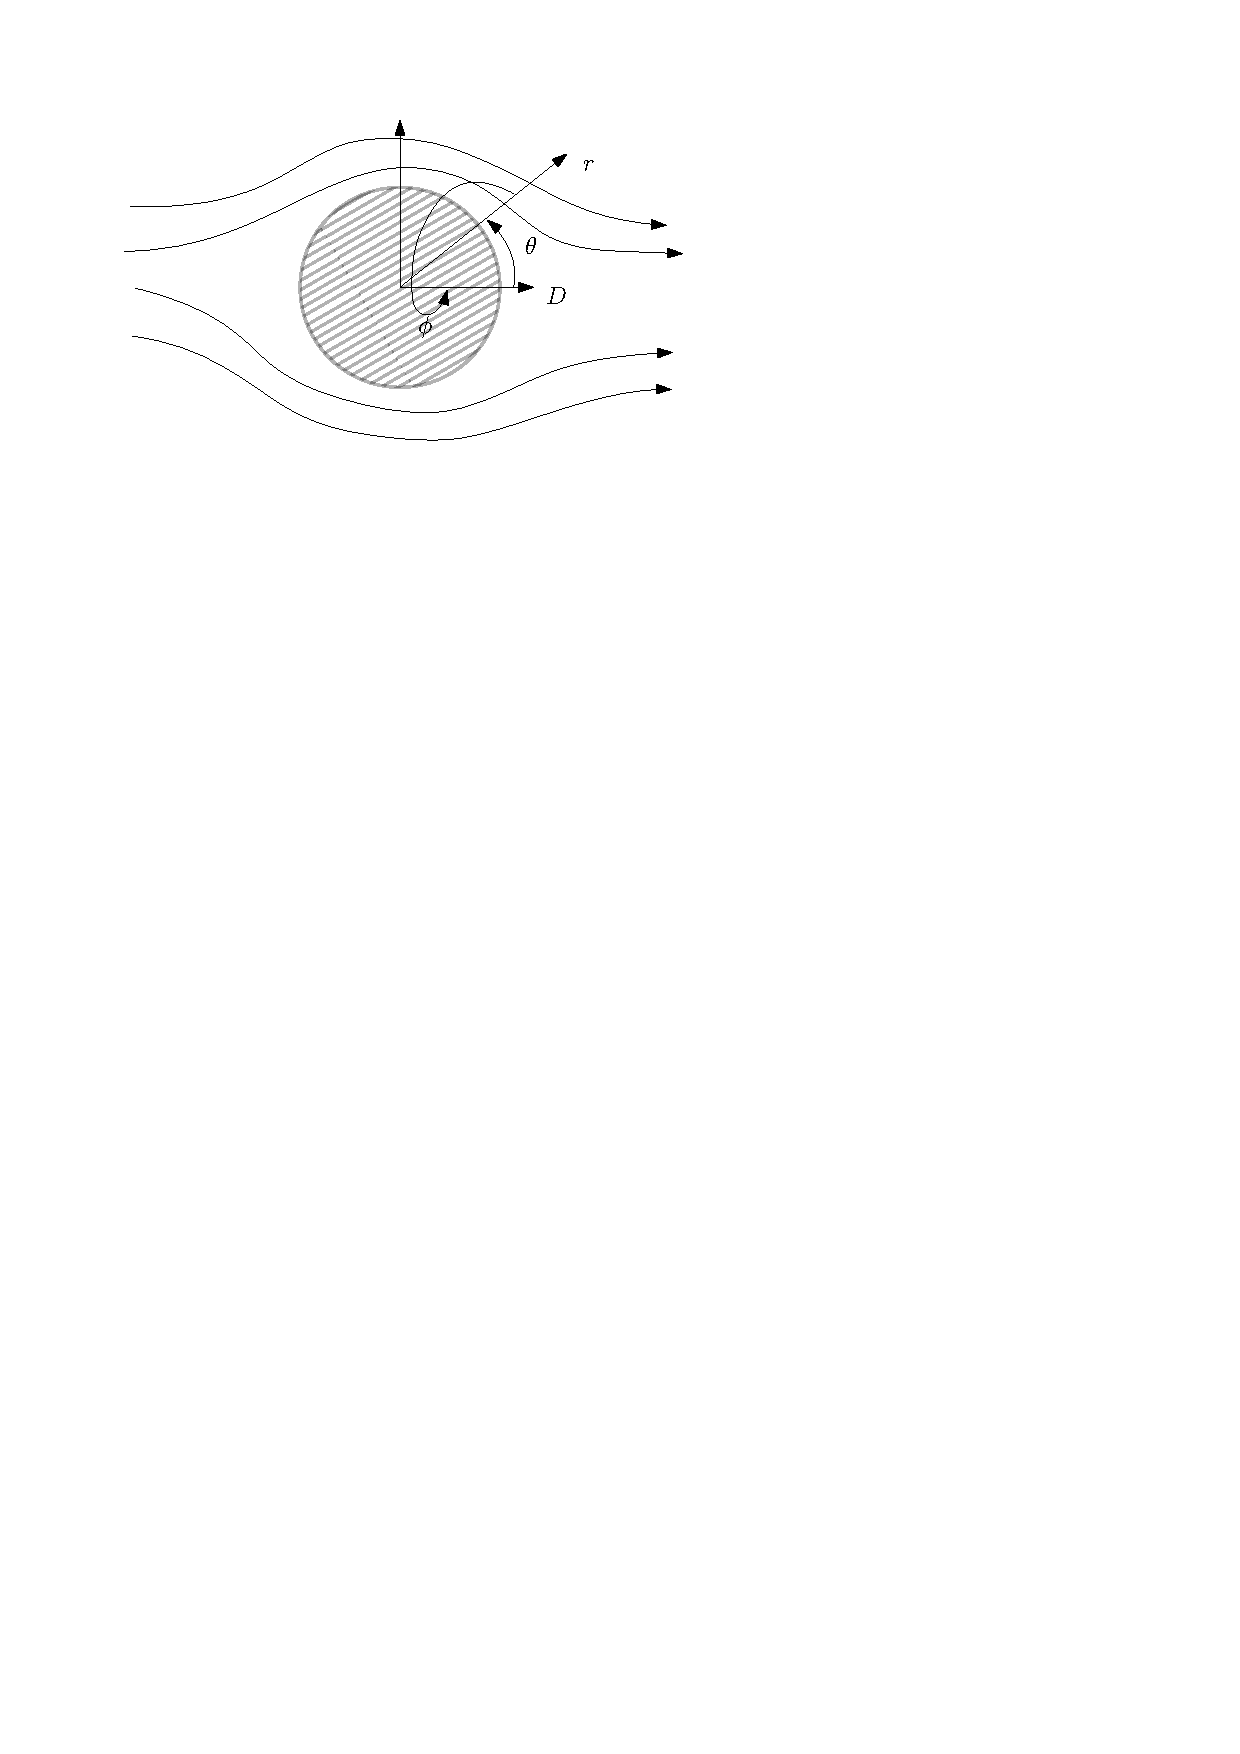
\includegraphics[scale=0.7]{./6.4 Correnti a basso numero di Reynolds/6.4-3}
		\centering
		\caption{Sfera in un fluido}
	\end{figure}
%
Si vede che anche per questo problema c'è una funzione di corrente del tipo:
%
	\begin{equation*}
		\psi = F(r) = \sin^2{\theta}
	\end{equation*}
%
Si risolve nuovamente il problema a variabili separabili, ma la soluzione è diversa, è del tipo:
%
	\begin{equation*}
		f = \frac{A}{r} + B r + C r^2 + D r^4
	\end{equation*}
%
La condizione sulla velocità ad infinito va con $r^2$, questo permette di determinare i coefficienti e risolvere il problema: per una sfera c'è un flusso di Stokes.
Si dimostra poi che la resistenza di una sfera è:
%
	\begin{equation*}
		F_D = 6 \pi \mu A U_{\infty}
	\end{equation*}
% 

\subsection*{Bibliografia 6.4}
\cite[Cap.\ 11.6]{CengelCimbala}\\
\cite[Cap.\ 9.3, 9.6]{PnueliGutfinger}